\section{Anwendungen}
Die Anwendung des NPR ist vielfältig: Strichzeichnungen sind im Bereich 
technischer Anleitungen oft besser verständlich als Fotos, auch in 
medizinischen Fachbüchern bilden Fotos eher eine Ausnahme. \par In anderen 
Bereichen, in denen es bisher üblich war, Zeichnungen von Hand anzufertigen, 
werden heute CAD- Programme eingesetzt. Um hierbei die selben Ergebnisse wie 
früher zu erreichen, ist oft ebenfalls NPR nötig (als Beispiel sei die 
Zeichnung von Architekten genannt, bei der der Detailgrad einer Strichzeichnung 
den Stand der Planung widerspiegelt). Ferner spielt NPR im künstlerischen 
Bereich und in Computerspielen eine große Rolle.

\subsection{Zeichentrickfilme}
Zeichentrickfilme oder Cartoons, kurze Filme die aus einer Aneinanderreihung 
von, zumeist handgezeichneten, Einzelbildern entstehen, werden heutzutage meist 
mit dem Computer produziert. Dabei werden 3D-Programme verwendet, die mit Hilfe 
eines Toon-Shaders die animierten Figuren so aussehen lassen, als seien sie von 
Hand gezeichnet. The Walt Disney Company, einer der größten Produzenten von 
Zeichentrickfilmen beschäftigt mittlerweile keinen einzigen Zeichner mehr, 
sondern setzt vollkommen auf die Computeranimation. Dabei wird vor allem der 
verringerte Aufwand sowie die schnellere Produktion und die geringeren Kosten 
gegenüber der handgezeichneten Variante als Vorteil genannt. Aber auch 
einfachere Umschnitte und Gegenperspektiven sowie Schwenks durch die Szenerie 
sind ein Vorteil der computerunterstützen Animation. Toon-Shader kommen meist 
nach dem Rendern zum Einsatz, in dem sie zunächst die Farbtiefe auf einige 
Zwischentöne reduzieren. Um schwarze Außenlinien zu produzieren, werden bei 
der Darstellung die Polygone einfach umgedreht und die schwarze Rückseite 
gezeichnet, meist mehrfach und leicht verschoben. Anschließend werden die 
Polygone wieder korrekt gezeichnet um Farbverläufe und optional auch Texturen 
darzustellen. Wird das Bild nun über den Z-Buffer zusammengesetzt, erscheinen 
die umgedrehten Polygone, welche immer tiefer sind als die anderen, als 
schwarze Konturen um die Objekte.

\subsection{Architektur}
Architekten verwenden gerne vereinfachende Verfahren der nicht-realistischen 
Computergraphik. Zu detailreiche Ansichten von Häusern oder anderen 
geometrischen Figuren überfordern den Kunden meist und werfen viele Fragen auf. 
Um diesem Problem zu begegnen verwenden Architekten oftmals einen reduzierten 
Bauplan und versuchen die Darstellung so weit zu abstrahieren, dass der Kunde 
gezwungen ist, die eigene Vorstellungskraft einzusetzen. Dies ist oft sehr 
hilfreich, da gerade die einfach gezeichneten Pläne leichter aufzunehmen sind 
und das Gehirn kann die Vorstellung besser in die reale Welt integrieren, als 
zu perfekt animierte Häuser, die den Eindruck erwecken, bereits gebaut worden 
zu sein. Vereinfachte Animationen helfen den Bauherren hingegen ihre 
Kreativität zu aktivieren und Raum für Veränderungen und Visionen zu geben.

\subsection{Maschinenbau}
Im Maschinenbau müssen oftmals Prinzipien die in komplexe Maschinen verpackt 
sind anschaulich erläutert werden. Ob in Bauplänen und Bedienungsanleitungen, 
oder in Forschungsberichten, die neuartige Prinzipien und deren Umsetzungen 
verdeutlichen sollen, es bleibt das Problem, dass vereinfachte Darstellungen 
von Modellen und Prinzipien verdeutlicht werden müssen. Da die reinen 
CAD-Zeichnungen absolut vollständig sind, ist es relativ schwer in ihnen die 
wichtigen Informationen zu erkennen. Um das unwichtige wegzulassen, generiert 
man hieraus gerne Explosions- oder Schnittzeichnungen (s.\ Abbildung 
\ref{fig:explosion}), die nur die wesentlichen Bestandteile zeigen. Andere 
Fälle sind beispielsweise halbtransparente Darstellungen von Automobilen, bei 
denen die Komponenten des Bremssystems hervorgehoben sind. Dies vereinfacht die 
Aufnahme in dem die Informationen auf das Wesentliche reduziert werden. In 
Bedienungsanleitungen wird auch gerne die Maschine als ganzes vereinfacht 
dargestellt, so dass man letztlich nur noch die Oberfläche der Mikrowelle 
darstellt, da dies absolut ausreichend ist, um ihre Bedienung zu erläutern.

\begin{figure}
  \centering
  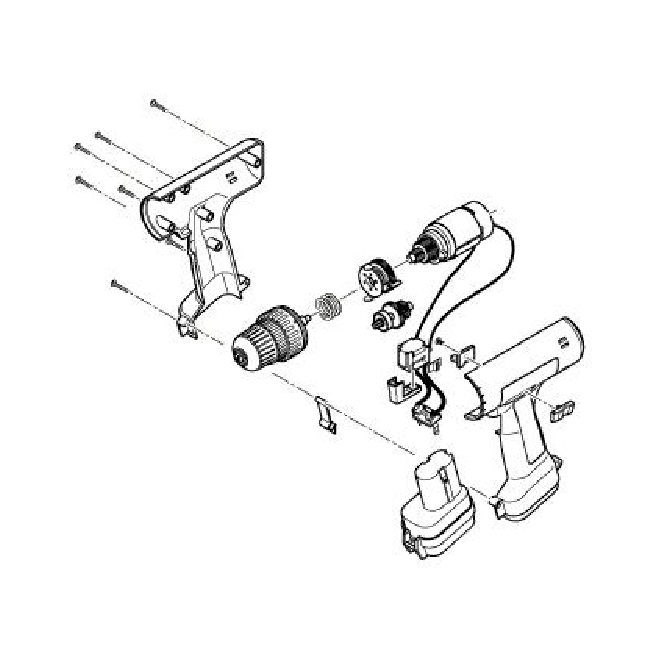
\includegraphics[width=0.5\textwidth]{../images/explosion}
  \caption{Beispiel für eine Explosionszeichnung}
  \label{fig:explosion}
\end{figure}

\subsection{Medizin}
Ebenso ist in der Medizin beispielsweise der Blutkreislauf oder ähnliches nicht 
einfach durch Fotos eines aufgeschnittenen Körpers darzustellen. Auch ein 
fotografiertes Herz enthält zu viele Details um als lehrreiche Skizze zu dienen.
 Generell kann man also der nichtrealistischen Computergraphik davon ausgehen, 
dass es sich um eine Designentscheidung handelt, die dem ungeübten Auge den 
Zugang zu Informationen durch Weglassung erleichtert.

\subsection{Biologie}
Ebenfalls ist in der Biologie weit verbreitet, Arten durch Skizzen einer 
Pflanze darzustellen. Diese beispielhaften Exemplare sind so in der Natur meist 
niemals zu finden, da sie in idealer Weise alle Merkmale in sich vereinen ohne 
zu viele Informationen darzustellen und so den Biologen zu verwirren. Es handelt
 sich also auch in diesem Fall um eine Unterstützung des Menschen durch 
Generalisierung der Merkmale einer Klasse von Pflanzen oder Tieren, die somit 
leichter wieder erkannt werden können. Zeichnete man diese Vorzeigekandidaten 
früher noch von Hand, übernimmt diese Arbeit nun oftmals der Computer. Es wäre 
einfach, eine realistische Pflanze zu erstellen die wie auf einem Foto 
aussieht. Die schwierigere Variante ist, die wichtigen Informationen 
herauszudestillieren und es so aussehen zu lassen, als wäre es eben diese 
abstrakte Repräsentation der Klasse von Pflanzen, um so dem Biologen die 
Möglichkeit der Klassifikation zu geben.

\subsection{Kartographie}
In der Kartographie versucht man ebenfalls viele Informationen auf einem 
kleinen Raum schematisch abstrahiert darzustellen. So finden sich 
beispielsweise Informationen über den Boden, das Klima, die Pflanzenwelt und 
Höheninformationen in der jeweiligen Farbzeichnung des Ausschnitts wieder. 
Erkennt man dies auf detailreichen Satellitenbildern ebenso gut? Sicherlich 
wäre ein Fachmann ohne Probleme dazu in der Lage, doch die vielen detailreichen 
Informationen würden einen Laien nur verwirren, könnte er sie überhaupt 
erkennen. Es muss also wieder zusammengefasst und abstrahiert werden, um die 
Informationen leicht zugänglich zu machen. Dieser Prozess ist keinesfalls 
einfach und darum kommen hier auch keine automatisierten Verfahren zum Einsatz, 
obwohl dies technisch durchaus möglich wäre. Aber um den Detailgrad richtig zu 
wählen und die Informationen präzise zu setzen muss ein Fachmann die 
Informationen filtern und viele Quellen zu einer einzigen Karte zu Rate ziehen. 
Diese Informationen werden nun zusammengeführt und schlagen sich beispielsweise 
in der Farbe der Erde an der jeweiligen Stelle nieder. Es kann durchaus sein, 
dass auf einer Karte der Alpen Schnee eingezeichnet ist, obwohl auf den 
Satellitenbildern der letzten 3 Jahre dort nachweislich kein Schnee gelegen 
hat. Aber über die Höhe und die Gegebenheiten ist nunmal entschieden worden, 
dass es eben generell möglich wäre, dass an dieser Stelle beispielsweise ein 
Gletscher entstehen kann. Ein weiteres Szenario ist die Simulation von 
Hochwasser und so die Möglichkeit hochwassergefährdete Gebiete einzuzeichnen 
obwohl hier eventuell noch nie ein Hochwasser in dieser Gegend war. Durch 
Physiksimulation der Landschaft sind diese Karten für die Bebauungsplanung aber 
ein wertvoller Hinweis, und sie können leicht von den zuständigen Behörden 
interpretiert werden, da die Informationen leicht zugänglich in der Karte über 
nicht-realistische Computergraphik dargestellt werden kann.